\documentclass[9pt,landscape]{article}
\usepackage{multicol}
\usepackage{calc}
\usepackage{ifthen}
\usepackage[landscape]{geometry}
\usepackage{amsmath,amsthm,amsfonts,amssymb}
\usepackage{color,graphicx,overpic}
\usepackage{hyperref}
\usepackage{wasysym}
\usepackage{mathtools}
\usepackage{tikz}
\usepackage{microtype}
\usetikzlibrary{arrows}
\usetikzlibrary{fit,positioning}

\pdfinfo{
  /Title (cheatsheet.pdf)
  /Creator (TeX)
  /Producer (pdfTeX 1.40.0)
  /Author (Chiel Kooijman)
  /Subject (Machine Learning 2 Cheat Sheet)
  /Keywords (pdflatex, latex,pdftex,tex)}

% This sets page margins to .5 inch if using letter paper, and to 1cm
% if using A4 paper. (This probably isn't strictly necessary.)
% If using another size paper, use default 1cm margins.
\ifthenelse{\lengthtest { \paperwidth = 11in}}
    { \geometry{top=.20in,left=.1in,right=.1in,bottom=.4in} }
    {\ifthenelse{ \lengthtest{ \paperwidth = 297mm}}
        {\geometry{top=1cm,left=1cm,right=1cm,bottom=1cm} }
        {\geometry{top=1cm,left=1cm,right=1cm,bottom=1cm} }
    }
% Turn off header and footer
\pagestyle{empty}

% Redefine section commands to use less space
\makeatletter
\renewcommand{\section}{\@startsection{section}{1}{0mm}%
                                {-0ex plus -.9ex minus -.5ex}%
                                {0.1ex plus .2ex}%x
                                {\normalfont\scriptsize\bfseries}}
\renewcommand{\subsection}{\@startsection{subsection}{2}{0mm}%
                                {-1explus -.5ex minus -.2ex}%
                                {0.1ex plus .2ex}%
                                {\normalfont\scriptsize\bfseries}}
\renewcommand{\subsubsection}{\@startsection{subsection}{2}{0mm}%
                                {-1explus -.5ex minus -.2ex}%
                                {0.1ex plus .2ex}%
                                {\normalfont\scriptsize\bfseries}}
\makeatother

% Define BibTeX command
\def\BibTeX{{\rm B\kern-.05em{\sc i\kern-.025em b}\kern-.08em
    T\kern-.1667em\lower.7ex\hbox{E}\kern-.125emX}}

\setlength{\parindent}{0pt}
\setlength{\parskip}{0pt plus 0.5ex}

%My Environments
\newtheorem{example}[section]{Example}
% -----------------------------------------------------------------------

\begin{document}
\footnotesize
\begin{multicols}{3}
% multicol parameters
% These lengths are set only within the two main columns
%\setlength{\columnseprule}{0.25pt}
\setlength{\premulticols}{1pt}
\setlength{\postmulticols}{1pt}
\setlength{\multicolsep}{1pt}
\setlength{\columnsep}{2pt}

\section{Distributions}
\begin{tabular}{l|lll}
\textbf{Binary} & Bernoulli & Binomial & Beta\\
\textbf{Discrete} & `categorical' & Multinomial & Dirichlet
\end{tabular}
\subsection{Bernouli}
$B(x|n) = \mu^x(1-\mu)^{1-x}$,
$E(x)=\mu$, $\mathrm{Var}(x) = \mu -\mu^2$,
$P(D,\mu) = \prod_{n=1}^N \mu^{x_n}(1 - \mu)^{1-x_n}$,
$\mu_{ML} = 1/N \sum_{n=1}^N x_n$

\subsection{Binomial}
$\mathrm{Bin}(x|N,\mu) = \binom{n}{k} \mu^m(1-\mu)^{N-m}$,
$\frac{n!}{k!(n-k)!} = \binom{n}{k}$,
$E(x) = N\mu$,
$\mathrm{Var}(x) = N\mu(1-\mu)$,
$\mu_{ML} = \frac{m}{N}$

\subsection{`categorical'}
$p(\vec{x}|\vec{\mu}) = \prod_{k} \mu_k^{x_k}$, $\mu = \left[0,1\right]^K$, $\sum_k \mu_k = 1$, $\vec{mu}_\mathrm{ML} = \frac{\vec{m}}{N}$, $m_k = \sum_n x_{nk}$
$\mathrm{Mult}(m_1 \ldots, m_k|N, \vec{\mu}) = (\frac{N!}{m_1!,\ldots, m_k} \prod_{k}) \mu_k^{mk}$
\subsection{Beta}
$\mathrm{Beta}(\mu|a,b) = \frac{\Gamma(a + b)}{\Gamma(a)\gamma(b)}\mu^{a-1}(1-\mu)^{b-1}$,
\footnote{
$\Gamma(x) = \int_0^1 u^{x-1}e^{-u} = 1$,
$\Gamma(x+1) = \Gamma(x)x$,
$\Gamma(x+1) = x!$
}
$E(\mu) = \frac{a}{a + b}$,
$\mathrm{Var}(x) = \frac{ab}{(a+b)^2(a+b+1)}$,
$p(\mu|m,l,a,b) \propto \mu^{m+a-1}(1-\mu)^{l+b-1}$

\subsection{Gamma Distribution}
$\mathrm{Gamma}(\tau | a,b) = \frac{b^a}{\Gamma(a)}\tau^{a-1}e^{-b\tau}$,
$E(\tau) = \frac{a}{b}$,
$\mathrm{Var}(\tau) = \frac{a}{b^2}$,
$\mathrm{mode}(\tau) = \frac{a-1}{b}$ for $a \ge 1$,
$E(\ln \tau) = \psi(a) - \ln b$,
$H(\tau) = ln \Gamma(a) - (a-1)\psi(a) - \ln b + a$

\subsection{Multinomial Distributions}
$\mathbf{x} = \lbrace 0,0,0,0,1,0,0 \rbrace^T$,
$\sum_{k=1}^K x_k = 1$,
$p(x|\mu) = \prod_{k=1}^K \mu_k^{x_k}$,
$\sum_{k=1}^K \mu_k = 1$,
$\mu_{ML} = \frac{m}{N}$,
$m_k = \sum_{k=1}^K x_{nk}$

\subsection{Dirichlet}
$\mathrm{Dir}(\mu|\alpha) = \frac{\Gamma(\sum_k a_k)}{\Gamma{a_1} \ldots \Gamma{a_k}} \prod_{k=1}^K\mu_k^{a_k-1}$

\subsection{Gaussian}
$\mathcal{N}(x|\mu,\sigma) = \frac{1}{\sqrt{2 \pi \sigma^2}}\exp(-\frac{1}{2\sigma^2}(x-\mu)^2)$,\\
$\mathcal{N}(x|\mu,\Sigma) = \frac{1}{(2\pi)^{D/2}} \frac{1}{\sqrt{|\Sigma|}} \exp(-\frac{1}{2}(x-\mu)^T) \Sigma^{-1} (x-\mu))$

\subsection{ML for the Gaussian}
$\ln p(X|\mu, \Sigma) = -\frac{ND}{2}\ln(2\pi) - \frac{N}{2}\ln|\Sigma| - \frac{1}{2}\sum_{n=1}^N (x_n - \mu)^T \Sigma^{-1} (x_n - \mu)$,
$\mu_{ML} = 1/N \sum_{n=1}^N x_n$,
$\Sigma_{ML} = 1/N \sum_{n=1}^N (x_n - \mu)^T (x_n - \mu)$

\subsubsection{Stochastic gradient descent Gaussian}
$\max\ P(x_1,...,x_n|\theta)$,
$\theta^N = \theta^{N-1} + \alpha_{N-1} \frac{\partial}{\partial \theta^{N-1}}
\ln\ p(x_n|\theta^{N-1})$

\subsection{Marginal and Conditional Gaussians}
Given $p(x) = \mathcal{N}(x | \mu, \Lambda^{-1})$ and $p(y|x) = \mathcal{N}(y | Ax + b, L^{-1})$. We get $p(y) = \mathcal{N}(y | A\mu + b, L^{-1} + A \Lambda^{-1} A^T)$ and $p(x|y) = \mathcal{N}(x | \Sigma\{ A^T L (y-b) + \Lambda \mu \}, \Sigma)$, where $\Sigma = (\Lambda + A^T L A)^{-1}$.

\subsection{Student's T distribution}
The heavy tail of the student-t distribution makes it more robust against outliers.\\
$St(x|\mu,\lambda,\nu) = \frac{\Gamma(\nu/2+1/2)}{\Gamma(\nu/2)}(\frac{\lambda^{1/2}}{(\pi \nu)^{D/2}}) [1+\frac{\lambda(x-\mu)^2}{\nu}]^{-\nu/2-D/2}$,\\
$f_{x}(x) = \frac{\Gamma[(\nu + p)/2]}{\Gamma(\nu/2) \nu^{p/2} \pi^{p/2}|\Sigma|^{1/2}[1 + 1/\nu(x-\mu)^T \Sigma^{-1}(x-\mu)]^{(\nu+p)/2}}$\\
$\mathbb{E}(\mathbf{x}) = \frac{\Gamma(D/2+v/2)}{\Gamma(v/2)} \frac{|\Lambda|^{1/2}}{(\pi v)^{D/2}} \int [1+\frac{(x-\mu)^T \Lambda (x-\mu)}{v}]^{-D/2-v/2}x\mathrm{d}x   $
\section{Graphical Models}
\textbf{GMs} are Robust, Capture noise, for reasoning, for when you have many variables (thousands), enormous data sets.
\textbf{Sidemark:} GMs are not like Neural Networks (NNs). A few reason are: NNs are models for supervised problems; a NN doesn't define a probabilistic model; transitions are not stochastic in a NN; a NN does not model conditional independence.


\subsection{Naive Bayes}
The Naive Bayes model assumes that given a label, all data cases are completely independent. (Percepron)
\subsection{Learning in a Bayes net}
The probability of a set of variables $\mathbf{x}$ in a Bayes Net is defined as
$p(x) = \prod_i p(x_i|x_{pa_i})$. If we define a function $\theta(x_i,
x_{pa_i})$ and use it instead of $p(x_i |x_{pa_i})$, we have $p(x) = \prod_i
\theta(x_i, x_{pa_i})$, if we constrain $\theta$ such that $\sum_{x_i}
\theta(x_i , x_{pa_i}) = 1, \forall i$.
We now have that the probability of the full data set:
$p(\{\widetilde x_{in}\}) = \prod_n \prod_i \prod_{x_i}
\prod_{x_{pa_{i}}} \theta(x_i, x_{pa_i})
^{\mathbb{I}[x_i = ̃\widetilde x_{in} \land x_{pa_i} = ̃\widetilde x_{pa_in}]}$

\subsection{Chain Rule}
$p(x_a,x_b,x_c) = p(x_c|x_a,x_b)p(x_b|x_a)p(x_a)$,
$p(x) = \prod_{k=1}^K p(x_k|{\mathrm{pa}_k})$
\subsection{DAGs}
No directed loops into the graph
\subsection{Markov chains}
A chain graph also called markov chain
\subsection{Discriminative}
$p(t|w) = p(w) \prod_{n=1}^N p(t_n|w)$
\subsection{Generative}
$T^* = P(T^*|W,X^*,X_i,T_i,\sigma^2,a)=$,
$[\prod_{i=1}^N P(X_i|W,\sigma^2)]$
$P(W|a)P(T^*|X^*,W,\sigma^2)$
\subsection{Misc}
$p(a,b|c) = p(a,b,c)/p(c)$,
$p(a,b,c) = p(a|c)p(b|c)p(c)$
\subsection{Markov Blanket}
\textbf{Directed case}: The MB of $x_i$ consists of : the parents of $x_i$, the
children of $x_i$ and the co-parents of the children of $x_i$.\\
\textbf{Undirected case}: All neighboring nodes of $x_i$.
\subsection{Blocking Rules}
$\Circle \rightarrow \CIRCLE \rightarrow \Circle$,
$\Circle \leftarrow \CIRCLE \rightarrow \Circle$,
$\displaystyle\Circle \rightarrow \cdots \Circle \cdots \leftarrow \Circle$
\subsection{Clique}
A set of nodes that is fully connected is called a clique. A maximal clique is a clique that cannot be made bigger.
\subsection{D-I-Perfect Map}
\textbf{D-Map:} A graph is said to be a D-map if every conditional independence statement satisfied by the distribution is reflected in the graph.\\
\textbf{I-Map:} If every conditional independence statement implied by the graph is satisfied by a specific distribution.\\
\textbf{Perfect Map:} If every conditional independence property is reflected in the graph and vise versa, then the graph is a perfect map.
\iffalse
\textbf{Hammersly-Clifford}
Define $\mathcal{UI}$ to be the set of such distributions that are consistent with the set of CIRs that can be read from the graph using graph separation. Define $\mathcal{UF}$ to be the set of such distributions that can be expressed as a factorization of the form $p(x) = \frac{1}{Z} \prod_C \phi_C (X_C)$ with respect to the maximal cliques of the graph. The Hammersly-Clifford theorem states that both sets are identical.
\fi
\subsection{Inference in Graphical Models}
\textbf{Bayes Theorem}: $p(x|y) = \frac{p(y|x)p(x)}{p(y)}$\\
\textbf{Inference on a chain}:\\
$p(x_1,\ldots,x_N)$\\
$ = \frac{1}{Z}\psi_{1,2}(x_1,x_2)\ldots\psi_{N-1,N}(x_{N-1},x_N)$\\
$ = \sum_{x_1}\sum_{x_2}\ldots\sum_{x_{N-1}}\sum_{x_N}p(x)$\\
$ = \sum_{x_1} \ldots \sum_{x_{n-1}} \sum_{x_{n+1}}\ldots \sum_{x_{N-1}} \sum_{x_{N}} p(x)$\\
$ = \frac{1}{Z}\sum_{x_1}\ldots\sum_{x_{n-1}}\psi_{x_1,x_2}\ldots \psi_{x_{n-1},x_n} \mu_\beta(x_n)$\\
$\mu_\beta(x_n) = \frac{1}{Z} \sum_{x_{n+1}}\psi_{x_{n},x_{n+1}} \ldots \sum_{x_N}\psi_{x_{N-1},x_{N}}$\\
$\mu_\alpha(x_n) = \frac{1}{Z} \sum_{x_{n-1}}\psi_{x_{n-1},x_{n}} \ldots \sum_{x_1}\psi_{x_{2},x_{1}}$\\
$p(x_n) = \frac{1}{z} \mu_\alpha(x_n) \mu_\beta(x_n)$, $O(NK^2)$

\subsection{Factor Graphs}
A tree is a graph with no loops. Both directed and undirected trees can be converted to a factor graph tree, but a directed tree could result in a non-tree structure when converted to an undirected representation. It is called a poly-tree (and not simply a tree) since its undirected representation (middle graph) includes a loop. The factor graph representation is again a tree. Factor graphs are the most general representation, and since any other tree representation can be easily converted to a factor tree, the sum-product algorithm is defined for factor trees.
\subsection{Sum-product algorithm}
Probability of the factor graph: $p(\vec{x}) = \frac{1}{Z}\prod_\alpha f_\alpha (\vec{x}_\alpha)$\\
\textbf{variable $\rightarrow$ factor message}
$\displaystyle \mu_{j\rightarrow \alpha}(x_j) = \prod_{\beta \in \mathrm{ne}(j)\smallsetminus\alpha} \mu_{\beta\rightarrow j}(x_j)$\\
\textbf{factor $\rightarrow$ variable message}
$\displaystyle \mu_{\alpha\rightarrow i}(x_i) = \sum_{x_{\alpha \smallsetminus i}}f_\alpha (\vec{x}_\alpha) \prod_{j\in \alpha \smallsetminus i}\mu_{j\rightarrow \alpha}$\\
\begin{tabular}{@{}llll}\\
\textbf{leaf node messages}&
$x_l$ & is a leaf node: & $\mu_{l\rightarrow \delta}(x_l) = 1$\\
&$\varepsilon$ & is a leaf node: & $\mu_{\varepsilon\rightarrow k}(x_k) = f_\varepsilon(x_k)$
\end{tabular}

\vspace{-1em}
\subsection{The max-sum algorithm}
$
\mathbf{x}^* = \arg \max_x \prod_a f_a(x_a)\\
p(\mathbf{x}^*) = \max_x \frac{1}{Z} \prod_a f_a(x_a)\\
\log p(\mathbf{x}^*) = \max_x -\log Z + \sum_a f_a(x_a)\\
$
\textbf{factor $\rightarrow$ variable message:}\\
$
v_{a \rightarrow i}(x_i) = \max_{x_a \setminus i} \left[ (\ln f_a(x_a)) + \sum_{j \in a \setminus i} v_{j \rightarrow a}(x_j) \right]
$\\
\textbf{variable $\rightarrow$ factor message:}\\
$
v_{j \rightarrow a}(x_j) = \sum_{\beta \in \mathrm{ne}(j) \setminus a} v_{\beta \rightarrow j}(x_j)\\
$
\vspace{-.5em}
\subsection{Variable Elimination}
\vspace{-.5em}
If we have some clusters $C_i$ and $C_j$, then:\\
$ S_{ij} = C_i \cap C_j $
Define potential functions $\Psi_i$ for each cluster $C_i$:
$ \forall C_i: \Psi_i \coloneqq \prod_{\psi_j \in C_i} \psi_j$
$ m_i \rightarrow C_j = \sum_{C_i \smallsetminus  S_{ij}} \Psi_i\prod_{k \in \mathrm{ne}(i) \smallsetminus j} m_{k \rightarrow i}(C_i)$\\
Note that:\\
$ C_i \setminus S_{ij} = C_i \setminus C_j $\\
Belief:\\
$ \Psi_{\text{root}} \prod_{k \in \mathrm{ne}(\text{root})} m_{k \rightarrow \text{root}}(C_{\text{root}}) \propto p(C_{\text{root}})$\\
Clusters replace factors, edges replace variables.\\
\textbf{Tree width} The width of a tree is one smaller than the biggest clique in the optimal ordering. Finding the optimal order is NP-hard.\\
\textbf{Running Intersection Property} A clique tree has the running intersection property if $x \in C_i \land x \in C_j \Rightarrow x \in C_k$ on the clique path between $C_i$ and $C_j$.

\vspace{.5em}
\section{learning/approx inference: EM (general), VEM, variational Bayes, Expectation Propagation}
\textbf{x,z, $\theta$} observed random, hidden random, parameters respectively.
The log-likelihood of the data is:
$
L(\theta) = \sum_n \log (\sum_z p(x_n,z_n|\theta))\\
=  \sum_n \sum_{z_n} q(z_n|x_n) \log \frac{p(x_n,z_n|\theta) q(z_n|x_n)}{q(z_n|x_n) p(z_n|x_n,\theta)}\\
= \log p(x_n|\theta)
$

\subsection{Variational EM Algorithm}
Variational EM algorithm has two steps:\\
 \textbf{E-Step:}\\
  \underline{Solve}
  $
  q_{t}(z_{n}|x_{n}) = p(z_{n}|x_{n},\theta_{t})\rightarrow B = l
  $
,(or increase $B(\theta_t, q)$ over $q$). This is not easy to solve, but sometimes it can be done (for example in Mixture of Gaussians).

It could be a situation where:\\
$
q(z|t) = \prod_{i=1}^k q(z|x)
$
The green dot upon the circle will be the best $q$ that approximates $p$ as it is the shortest point from $p$.

\textbf{M-Step:}\\
\underline{Solve}
$
{t+1} = \arg\max_{\theta} \sum_{n} Eq_{t}[\log p(x_{n},z_{n}|\theta)]
$
, (or increase $B(\theta,q_{t})$ over $\theta$). Implicitly, $\theta$ is in that $q_{t}$ of the expectation because it is \underline{fixed} from the previous iteration. We maximize the lower bounds until we find the maximum. The convergence is rather slow. In terms of speed is not the best algorithm.\\
\underline{Proof of Convergence:}\\
We have to prove that:
$
h(\theta_{t}) \leq \ldots \leq h(\theta_{t+1})
$

$
 h(\theta_{t}) = B(\theta_{t},p(z|x,\theta_{t}))
$
$
h(\theta_{t}) \leq B(\theta_{t+1},p(z|x,\theta_{t}))
$
, (M-Step): We maximise over $\theta_{t+1}$. So $B$ in eq.(13) must be bigger than the one in the (12). In the next step we have:
$
h(\theta_{t}) = l(\theta_{t+1})-\mathcal{KL}[q_{t}||p(z|x,\theta_{t+1})]
$
, (l=B+$\mathcal{KL}$) The distribution in Kullback-Leibler divergence are not
the same so $\mathcal{KL}$ is not equal to $0$ at this occasion, due to the
fact that the two terms of $\mathcal{KL}$ divergence are coming from different iterations. Hence,
$
h(\theta_{t}) \leq h(\theta_{t+1})
$
, cause $\mathcal{KL} \geq 0$.\\
\textbf{Lower bound $\mathcal{L}(q)$ and KL-divergence}
$\text{ln } p(X) = \mathcal{L}(q) + KL(q||p)$\\
$\mathcal{L} (q) = \int q(Z) \text{ln } \big\{ \frac{p(X,Z)}{q(Z)} \big\} dZ$ \\
$KL(q||p) = - \int q(Z) \text{ln } \big \{ \frac{p(Z|X)}{q(Z)} \big\} dZ$\\
\textbf{Note that}\\
$Q(\theta,\theta^{old}) = \sum_z p(Z|X,\theta^{old}) \text{ln } p(X,Z|\theta) = \mathbb{E}_{Z|X,\theta^{old}}[\text{ln } p(X,Z|\theta)]$

\subsection{Expectation Propagation}
Joint distribution $p(D,\theta) = \prod_i f_i(\theta)$\\
Approximate $p(\theta|D)$ using $q(\theta) = \frac{1}{Z} \prod_i \tilde f_i(\theta)$, and also approximate $p(D)$ somehow.\\
\begin{enumerate}
\item Initialize approximating factors $\tilde f_i(\theta)$
\item Initialize the posterior approximation by setting $q(\theta)\varpropto \prod_i \tilde f_i(\theta)$
\item Until convergence:
\begin{enumerate}
\item Choose a factor $\tilde f_j(\theta)$ to refine
\item Remove $\tilde f_j(\theta)$ from the posterior by division: $q^{\setminus j}(\theta) = \frac{q(\theta)}{\tilde f_j(\theta}$
\item Evaluate new posterior by setting the moments of $q^{new}(\theta)$ equal to those of $q^{\setminus j}(\theta) f_j(\theta) d\theta$, including $Z_j = \int q^{\setminus j} (\theta) f_j(\theta) d\theta$
\item Evaluate + store new factor $\tilde f_j(\theta) = Z_j \frac{q^{new}(\theta)}{q^{\setminus j})\theta}$
\end{enumerate}
\item Evaluate the approximation to the model evidence $p(D) \simeq \int \prod_i \tilde f_i(\theta) d\theta$
\end{enumerate}


\section{sampling: standard, MCMC, Gibbs, HybridMC}
\subsection{Rejection sampling}
We take a $q(z)$ distribution, choose k for $kq(z) \geq p(z),e z \in p(z)$\\
$p(accepted) = \int \lbrace p(z)/kq(z) \rbrace q(z) \mathrm{d}z
= \frac{1}{K} \int p(z) \mathrm{d}z$
\subsection{Adaptive rejection sampling}
When we have a distribution $p(z)$ where $\ln p(z)$ has derivatives which are not increasing functions of z. The envelope distribution is a succession of linear functions.
$q(z) = k_i \lambda_i \exp \lbrace -\lambda_i (z-z_i) \rbrace$.
Then rejection sampling can be applied.
\subsection{Importance sampling}
Provides a framework for approximating distributions but does not provide a mechanism for drawing samples from them.
Used when it is not easy to find a function that forms an upper bound. Note
that q does not necessarily have to be a bound on p, as we weigh by the quotient of the two distributions. Samples are drawn from distribution q and weighed correspondingly:
$x_i \approx \tilde{q}$, $w_i = \frac{\tilde{p}(x_i)}{\tilde{q}(x_i)}$
Works bad in high dimensions as it is hard to find an x where both q(x) and p(x) are
high in the high-dimensional space. If p and q overlap just a little, this will give a bad
estimate.

\subsection{Ancestral sampling AKA Likelihood Weighted sampling}
Given a Bayesian network, we can write down the joint probability as $p(z1)p(z2|z1)$. That means there is always a node in the tree that is not dependent on any other variable.
We sample this node, and use the sample to draw samples for subsequent nodes. If we observe values ($x \in Ev$, evidences), we just select the observed value instead of
sampling. Works bad in high dimensions as well.

\subsection{Markov Chain Monte-Carlo (MCMC) sampling}
MCMC runs ancestral sampling on a chain. Samples can no longer be drawn independently.
$t \rightarrow 1$, $x_t \sim q_{\infty}(x_{\infty})$ Equilibrium or invariant distribution. We transition from $q_1$ to $q_2$ according to transition probability $T(x_2|x_1)$.\\
$q(x_{t+1}, x_t) = T(x_{t+1}|x_t)q(x_t)$\\
\textbf{Invariance}:
We want to find T for a given p, such that $p = T p$ holds.\\
\textbf{Detailed balance}:(or reversibility) We want to find T so that transition from one state to another has probability mass equal to the transition from that next state to the current. Thus, $p^*(z)T(z,z') = p^*(z')T(z',z)$. Distribution $p^*(z)$ is invariant if $p^*(z)=\sum_{z'}p^*(z')T(z',z)$\\ Proof:$A_k(z',z) = \text{min }\big( 1, \frac{p(z')q(z|z')}{p(z)q(z'|z)} \big)$\\
$p(z)q(z'|z)A_k(z',z) = \text{min } \big( p(z)q(z'|z),p(z')q(z|z') \big)$ [multiply by denom]\\
$= \text{min }\big(p(z')q(z|z'), p(z)q(z'|z) \big)$ [order irrelevant]\\
$= p(z')q(z|z')A_k(z,z')$
\textbf{Ergodicity}:
This algorithm needs ergodicity: A positive probability for every state (so all will be reached).\\
\textit{For two transition kernels $T_1, T_2$ that are valid any linear combination of these two is a valid kernel.}

\subsection{Metropolis-Hastings algorithm}
In the $\tau$ step of the algorithm the current state is $z^{(\tau)}$, we draw sample $z^*$ from $q_k(z|z^{(\tau)})$, which it is been accepted with probability: $ A_k(z^*,z^{(\tau)}) =\min (1, \frac{p(z^*) q_k(z^{(\tau)}|z^*)}{p(z^{(\tau)}) q_k(z^*|z^{(\tau)})}) $, where k labels the set of possible transitions. Metropolis-Hastings algorithm work better in high dimensions than previous methods, but is quite slow (as we perform a random walk).


\subsection{Quasi-MC sampling}
Fun fact: If we sample in a smart way (e.g. not sample the same point twice, ensure that areas there hasn't been sampled from have higher probability of being chosen) instead of random, these methods may converge faster.

\subsection{Gibbs sampling}
For a distribution $p(\mathbf{z})$, for each component of the distribution $z_i$ draw a sample from the distribution of that variable given the values of the remaining variables:
\begin{enumerate}
\item Initialize $\{ z_i: i = 1, \dots ,M$
\item For $\tau = 1,\dots ,T$:
\begin{itemize}
  \item Sample $z_1^{\tau+1} \sim p(z_1|z_2^{\tau},\dots , z_M^{\tau})$\\
  $\vdots$
  \item Sample $z_j^{\tau+1} \sim p(z_j|z_1^{\tau+1},\dots ,z_{j-1}^{\tau+1},z_{j+1}^{\tau},\dots , z_M^{\tau})$\\
  $\vdots$
  \item Sample $z_M^{\tau+1} \sim p(z_M|z_1^{\tau+1}, \dots ,z_{M-1}^{\tau+1}$
\end{itemize}
\end{enumerate}

\subsection{Algorithm Hamiltinian MC (HMC)}
Energy $H$ is conserved.
\begin{enumerate}
\itemsep0em
\item $x \sim p(x) = \frac{1}{z} e^{-H(x)}$
\item $\mathbf{x_0}$
\item draw $r_0 \sim \mathcal{N}(0,1)$
\item ``Leapfrog stepping''
\begin{itemize}
\itemsep0em
\item $r_i (t+ \frac{\epsilon}{2}) = r_i(t) - \frac{\epsilon}{2} \frac{\partial E}{\partial x_i}|_{x_{i{(t)}}}$
\item $x_i(t+\epsilon) = x_i(t) + \epsilon r_i (t+\frac{\epsilon}{2})$
\item $r_i(t+\epsilon) = r_i (t+\frac{\epsilon}{2}) -\frac{\epsilon}{2}\frac{\partial E}{\partial x_i}|_{x_{i{(t+\epsilon)}}}$
\item Iterate for T rounds.
\end{itemize}
\item Accept $(x(t), r(t))$, with probability $\alpha = \min (1, e^{H_0-H_t})$.
\item Repeat
\end{enumerate}
Regarding step 4, it must be noted that the acceptance probability would always be
1 if the Hamiltonian dynamics would be modelled perfectly (i.e. $H_t = H_0$). However, in
practice this is not the case due to numerical errors.

\section{HMMs + Kalman filters}
\vspace{-.4em}
\subsection{Markov models}
\vspace{-.4em}
First order Markov chains hold the Markov property which you whole history is only dependent on the current state. \textbf{First order}'s number of parameters will be: $k-1+k(k-1)$. \textbf{Second order}: $k^2-1+k^2(k-1)$.

\vspace{-.4em}
\subsection{HMMs}
\vspace{-.4em}
Useful in speech recognition, natural language processing, online character recognition...
Discrete variables: HMM, Linear-Gaussian: LDS (Linear Dynamical System).\\
$p(x,\ldots, x_n) = \sum_{z_1} \ldots \sum_{z_n}p(z_1)(\prod_{n=2}^N p(z_n|z_{n-1},A))\prod_{n=1} p(x_n|z_n)$\\
For the first node:\\
$p(z_1|\pi) = \prod_{k=1}^K \pi_k^{z_{1,k}}$\\
$p(z_n|z_{n-1},A) = \prod_{k=1}^K \prod_{j=1}^K A_{jk}^{z_{n-1},jz_{nk}}$\\
$p(x_n|z_n,\phi) = \prod_{k=1}^K p(x_n|\phi_k)^{z_{nk}}$\\
Where A, $\phi$ and $\pi$ are the parameters of the model. $p(x_n|z_n,\phi)$ is model-dependent
(e.g.: mixture of Gaussians, multinomial if discrete, etc).
\vspace{-.4em}
\subsubsection{Maximum likelihood (EM)}
\vspace{-.4em}
data: X, latent state: Z, parameters: $\theta = (\pi, A, \phi)$.\\
$p(x|\theta) = \sum_z p (x,z|\theta)$\\
This represents a sum of KN terms, which quickly becomes intractable, so we can use
for instance the EM algorithm.\\
\textbf{E-step:}\\
$Q(\theta|\theta^{old}) = \sum_z p (z|x,\theta^{old})\ln p (x,z|\theta)$\\
\textbf{M-step:}\\
$\theta^{new} = \arg\max_{\theta}Q(\theta|\theta^{old})$\\
EM-general:\\
$\ln p(X|\theta) = \mathcal{L}(q, \theta) + \mathcal{KL}(q||p)$ where
$\mathcal{L}(q, \theta) = \sum_Z q(Z) \ln(\frac{p(X, Z| \theta)}{ q(Z)})$ and
$\mathcal{KL}(q||p) = -\sum_Z q(Z) \ln(\frac{p(Z| X, \theta)}{q(Z)})$.\\
E-step: maximize $\mathcal{L}(q, \theta)$ wrt $q(Z)$. M-step: maximize $\mathcal{L}(q, \theta)$ wrt $\theta$.

\subsubsection{Forward-Backward}
$$a(z_n) = p(x_n|z_n) \sum_{z_{n-1}} a(z_{n-1})p(z_n|z_{n-1})$$
$$\beta(z_n) = \sum_{z_{n+1}} \beta(z_{n+1}) p(x_{n=1}|z_{n+1})p(z_{n+1}|z_n)$$
\textbf{Predictive distribution}: Add $x_{n+1}$ and $z_{n+1}$ at the end of the chain and use the calculated parameters to predict the new values.(assuming the chain is homogeneous). By d-separation (if applicable), $p(x_{N+1}|X) = p(x_{N+1}|x_{N})$ (regular Markov Chain, add $z$'s to taste. 
\section{Causality}
\begin{scriptsize}
\textbf{Statistics}, (most of) Machine Learning
About associations (correlation between chocolate consumption and
winning a Nobel prize), Models the distribution of the data. Predicting by conditioning (if we observe that somebody eats much
chocolate, what is the probability that he/she will win a Nobel prize?)
\textbf{Causality}, About causation (does chocolate consumption cause winning a Nobel
prize?), Models the mechanism that generates the data. Predicting results of interventions (if we force somebody to eat a lot
of chocolate, what is the probability that he/she will win a Nobel
prize?)
$$p(y,x) \neq p(y|\mathrm{do}(x))$$
The causal model playing violent computer games causes violence
may be formalized as a linear model:
$V = \beta G$
We summarize the in
influence of all ``other causes of V'' with a single variable E: $V = \beta G +E$. V and G are endogenous variables, E is an exogenous variable.
By assumption, exogenous variables are not caused by endogenous
variables (although they may cause endogenous variables).
Endogenous variables are usually observed; exogenous variables are
usually unobserved (latent, hidden).
\end{scriptsize}
\subsection{Structural causal models}
A Structural Causal Model (SCM) is defined by:
\begin{itemize}
\item $X^{(N)}$ endogenous and $E^{(N)}$ exogenous random variables.
\item $X_i^{(N), \text{effect}} = f^\text{causal.Mech}_i(X^\text{direct.Cause}_{pa(i)}, E_i^\text{noise})$
\item A joint prob distr. $p(E_1,\ldots, E_N)$
\end{itemize}
Directed arrows correspond with
functional dependences and are interpreted as direct causal relations. An \textbf{intervention} $do(XI = I)$ on a set of variables \textbf{X}, forcing them to attain the value $\xi$. \texttt{The effect of the intervention is to remove all incoming arrows of intervened variables.}\\
\textbf{Causal feedback} if a graph contains a directed cycle, acyclic otherwise.\\
A \textbf{confounder} is an unobserved variable that is an ancestor of at least two
endogenous variables.\\
If all exogenous variables in an SCM are jointly independent then we say that the endogenous variables X are \textbf{causally sufficient}.\\
An SCM M is called \textbf{Markovian} if:\\
$\rightarrow$ it is acyclic\\
$\rightarrow$ it is causally sufficient.\\
\textbf{Causal Markov Condition/Truncated Factorization:}\\
$p(x_1, \ldots, x_N) = \prod_{i=1}^N p(x_i|x_{pa(i)})$\\
\textbf{After an intervention:}\\
$p(x_1, \ldots, x_N|do(x_l=\psi_l)) = \prod_{i=1\\;i\not\in l}^N p(x_i|X_{pa(i)}) \prod_{i\in l} \mathbf{I}[x_i = \psi_i]$
\textit{Each Markovian SCM induces a Bayesian network. Conversely, for any given Bayesian network, one can construct a
Markovian SCM that induces the same probability distribution.
We prefer SCMs over Bayesian Networks because they generalize to
non-Markovian situations.}
\subsection{Back-door criterion}
Let G be a graph with directed and bidirected  edges.\\
A \textbf{path} q is a sequence of distinct consecutive edges (where the end
node of each edge equals the start node of the next edge).\\
A \textbf{collider} on a path q is a node X on q with precisely two
``incoming'' arrow heads.\\
Given a path p
between nodes X and Y in G: we saythat S \textbf{blocks} p if p contains:\\
a \textbf{non-collider} which is in S or\\
a \textbf{collider} which is not an \textbf{ancestor} of S.\\
\textbf{Theorem: Back-door criterion}
\begin{enumerate}
\item No element of S is a descendant of X
\item The elements of S block all back-door paths $X \leftarrow \ldots Y$ and
$X \leftrightarrow \ldots Y$ (paths between X and Y with an arrow pointing to X).
\end{enumerate}
In that case:
$p(Y|do(X)) = \int p(Y|X,X_s)p(X_s) \mathrm{d}X_s$

\section{Homework}
\subsection{Derive the mean, covariance, and mode of multivariate Student's t-distribution.}
$\mathbb{E}[x], z = (x - \mu), \int \ldots z \mathrm{d}z = 0,odd,result=\mu$\\
$\mathbb{E}[x-\mu], z = (x - \mu), \int \ldots z \mathrm{d}z = 0,odd,result=0$

\subsection*{Chi-squared distribution with n degrees of freedom}
The normal distribution's density function is given by:
$
f(x) = \frac{1}{\sqrt{2\pi\sigma^2}}e^{\frac{-(x-\mu)^2}{2\sigma^2}}
$
Given that $g(T|V=v) =\mathcal{N}(0,\frac{n}{v})$, we can write $z(t)$ as:
$
z(t) = \frac{1}{\sqrt{2\pi\frac{n}{v}}}e^{\frac{-t^2}{2 \frac{n}{v}}}
 = \frac{1}{\sqrt{2\pi\frac{n}{v}}}e^{\frac{-vt^2}{2 n}}
$
Also, for the chi-squared distribution we have:
$
f(x) = \frac{1}{2^{\frac{n}{2}}\Gamma(\frac{n}{2})}x^{\frac{n}{2} - 1}e^{\frac{-x}{2}},\ x=v \Leftrightarrow\\
f(v) = \frac{1}{2^{\frac{n}{2}}\Gamma(\frac{n}{2})}v^{\frac{n}{2} - 1}e^{\frac{-v}{2}}
$
Due to the fact that $Z$,$V$ independent, we can compute their joint probability density function. Lets denote another distribution which is the multiplication of $z,f$, $g(t,v) = z(t) \times f(v)$.
$
g(t,v) = z(t) \times f(v)\\
=\frac{1}{\sqrt{2\pi\frac{n}{v}}}e^{\frac{-vt^2}{2 n}} \frac{1}{2^{\frac{n}{2}}\Gamma(\frac{n}{2})}v^{\frac{n}{2} - 1}e^{\frac{-v}{2}}
=\frac{1}{2^{\frac{n}{2n}} \sqrt{2\pi n}\Gamma(\frac{n}{2})}v^{\frac{1}{2}(n-1)} e^{-\frac{v}{2n}(t^2+n)}\\
$
Now, we can find its probability density function integrating in respect to $v$:
$
pdf = \int_0^\infty \frac{1}{2^{\frac{n}{2}} \sqrt{2\pi n}\Gamma(\frac{n}{2})}v^{\frac{1}{2}(n-1)} e^{-\frac{v}{2n}(t^2+n)} \mathrm{d}v \\
= \frac{1}{2^{\frac{n}{2}} \sqrt{2\pi n}\Gamma(\frac{n}{2})} \int_0^\infty v^{\frac{1}{2}(n-1)} e^{-\frac{v}{2n}(t^2+n)} \mathrm{d}v
$
We know that:
$
\int_0^\infty x^n e^{-ax} \mathrm{d}x = \frac{\Gamma(n+1)}{a^{n+1}}
$
In eq. 29 we have:
$
a = \frac{1}{2n}(t^2+n),\ n = \frac{1}{2}(n-1)
$
Replacing in a we have:
$
= \frac{\Gamma(\frac{1}{2}(n-1)+1)}{2^{\frac{n}{2}} \sqrt{2\pi n}\Gamma(\frac{n}{2}) (\frac{1}{2n}(t^2+n))^{\frac{1}{2}(n-1)+1}}
= \frac{\Gamma(\frac{n+1}{2})}{\sqrt{\pi n}\Gamma(\frac{n}{2})} (1 + \frac{t^2}{n})^{-\frac{n+1}{2}}
$
, which is the probability density function of student's t-distribution.

\subsection{$\mathcal{KL}$ divergence of two Gaussians}
Given the distributions p and q of a continuous random variable, Kullback-Leibler divergence of q from p is:
$
\mathcal{K}\mathcal{L}(p||q) = - \int p(\mathbf{x}) \ln \lbrace \frac{q(x)}{p(x)} \rbrace \text{d}x,\	\text{matrix.cook.(324)} \\
= - \int p(\mathbf{x}) \ln \lbrace \frac{\frac{1}{\sqrt{\det(2 \pi \mathbf{\Sigma})}} \exp[{{-\frac{1}{2}(\mathbf{x} - \mathbf{\mu})^T \mathbf{\Sigma}^{-1} (\mathbf{x} - \mathbf{\mu})]}}}{\frac{1}{\sqrt{\det(2 \pi \mathbf{L})}} \exp[{{-\frac{1}{2}(\mathbf{x} - \mathbf{m})^T \mathbf{L}^{-1} (\mathbf{x} - \mathbf{m})]}}} \rbrace \text{d}\mathbf{x}\\
= - \int p(\mathbf{x}) \ln \lbrace \frac{\frac{1}{\sqrt{\det(2 \pi \mathbf{\Sigma})}}}{\frac{1}{\sqrt{\det(2 \pi \mathbf{L})}}} \rbrace
\ln \lbrace \frac{\exp[{{-\frac{1}{2}(\mathbf{x} - \mathbf{\mu})^T \mathbf{\Sigma}^{-1} (\mathbf{x} - \mathbf{\mu})}}]}{\exp[{{-\frac{1}{2}(\mathbf{x} - \mathbf{m})^T \mathbf{L}^{-1} (\mathbf{x} - \mathbf{m})}}]} \rbrace \mathrm{d}\mathbf{x}\\
= - \int p(\mathbf{x}) \ln \lbrace \frac{\mathbf{L}}{\mathbf{\Sigma}} \rbrace^{1/2}
ln \lbrace \exp[-\frac{1}{2}(\mathbf{x} - \mathbf{\mu})^T \mathbf{\Sigma}^{-1} (\mathbf{x} - \mathbf{\mu}) + \frac{1}{2}(\mathbf{x} - \mathbf{m})^T \mathbf{L}^{-1} (\mathbf{x} - \mathbf{m})] \rbrace \mathrm{d}\mathbf{x}\\
= - \int p(\mathbf{x}) \ln \lbrace \frac{\mathbf{L}}{\mathbf{\Sigma}} \rbrace^{1/2}
( -\frac{1}{2}(\mathbf{x} - \mathbf{\mu})^T \mathbf{\Sigma}^{-1} (\mathbf{x} - \mathbf{\mu}) + \frac{1}{2}(\mathbf{x} - \mathbf{m})^T \mathbf{L}^{-1} (\mathbf{x} - \mathbf{m}) ) \mathrm{d}\mathbf{x}\\
= -\frac{1}{2}\ln \lbrace \frac{\mathbf{L}}{\mathbf{\Sigma}} \rbrace \int p(\mathbf{x})  
( -\frac{1}{2}(\mathbf{x} - \mathbf{\mu})^T \mathbf{\Sigma}^{-1} (\mathbf{x} - \mathbf{\mu})) \mathrm{d}\mathbf{x} + \int p(x)(\frac{1}{2}(\mathbf{x} - \mathbf{m})^T \mathbf{L}^{-1} (\mathbf{x} - \mathbf{m}) \mathrm{d}\mathbf{x}\\
= -\frac{1}{2}\ln \lbrace \frac{\mathbf{L}}{\mathbf{\Sigma}} \rbrace( \mathrm{E}
( -\frac{1}{2}(\mathbf{x} - \mathbf{\mu})^T \mathbf{\Sigma}^{-1} (\mathbf{x} - \mathbf{\mu})) + \mathrm{E}(\frac{1}{2}(\mathbf{x} - \mathbf{m})^T \mathbf{L}^{-1} (\mathbf{x} - \mathbf{m})),\	\text{matrix.cook.(357)}\\
= -\frac{1}{2}\ln \lbrace \frac{\mathbf{L}}{\mathbf{\Sigma}} \rbrace( -\frac{1}{2}((\mathbf{\mu} - \mathbf{\mu})^T \mathbf{\Sigma}^{-1} (\mathbf{\mu} - \mathbf{\mu}) + \mathrm{Tr}(\mathbf{\Sigma}\mathbf{\Sigma}^{-1}))) + \frac{1}{2}((\mathbf{\mu} - \mathbf{m})^T \mathbf{\Sigma}^{-1} (\mathbf{\mu} - \mathbf{m}) + \mathrm{Tr}(\mathbf{\Sigma}\mathbf{L}^{-1}))))\\
= -\frac{1}{2}\ln \lbrace \frac{\mathbf{L}}{\mathbf{\Sigma}} \rbrace( -\frac{1}{2}\mathrm{Tr}(\mathbf{\Sigma}\mathbf{\Sigma}^{-1}) + \frac{1}{2}((\mathbf{\mu} - \mathbf{m})^T \mathbf{\Sigma}^{-1} (\mathbf{\mu} - \mathbf{m}) + \mathrm{Tr}(\mathbf{\Sigma}\mathbf{L}^{-1})))
$

\subsection{Entropy of Gaussian}
$
H(x) = - \int p(x) \ln (p(x)) \mathrm{d}\mathbf{x}\\
= - \int p(x) \ln (\frac{1}{\sqrt{\det(2 \pi \mathbf{\Sigma})}} \exp[{{-\frac{1}{2}(\mathbf{x} - \mathbf{\mu})^T \mathbf{\Sigma}^{-1} (\mathbf{x} - \mathbf{\mu})]}})\mathrm{d}\mathbf{x}\\
= - \int p(x) [-\ln(2\pi)^{d/2} - \frac{1}{2}\ln|\Sigma|- \frac{1}{2}(\mathbf{x} - \mathbf{\mu})^T\mathbf{\Sigma}^{-1}(\mathbf{x} - \mathbf{\mu})]\mathrm{d}\mathbf{x}\\
= \int p(x) [ \ln(2\pi)^{d/2} + \frac{1}{2}\ln|\Sigma|+ \frac{1}{2}(\mathbf{x} - \mathbf{\mu})^T\mathbf{\Sigma}^{-1}(\mathbf{x} - \mathbf{\mu})] \mathbf{d}\mathbf{x}\\
= \int p(x) \ln(2\pi)^{d/2}  \mathrm{d}\mathbf{x} + \int p(x) \frac{1}{2}\ln|\Sigma| \mathrm{d}\mathbf{x} + \int p(x) \frac{1}{2}(\mathbf{x} - \mathbf{\mu})^T\mathbf{\Sigma}^{-1}(\mathbf{x} - \mathbf{\mu}) \mathrm{d}\mathbf{x}\\
= \frac{d}{2} \int p(x) \ln(2\pi)  \mathrm{d}\mathbf{x} + \frac{1}{2} \int p(x)\ln|\Sigma| \mathrm{d}\mathbf{x} + \frac{1}{2} \int p(x) (\mathbf{x} - \mathbf{\mu})^T\mathbf{\Sigma}^{-1}(\mathbf{x} - \mathbf{\mu}) \mathrm{d}\mathbf{x}\\
= \frac{d}{2} \mathrm{E}(\ln(2\pi)) + \frac{1}{2} \mathrm{E}(\ln|\Sigma|) + \frac{1}{2} \mathrm{E}(\mathbf{x} - \mathbf{\mu})^T\mathbf{\Sigma}^{-1}(\mathbf{x} - \mathbf{\mu})\\
= \frac{d}{2} \ln(2\pi) + \frac{1}{2} \ln|\Sigma| + \frac{1}{2} d\\
= \frac{d}{2}(\ln(2\pi)+1) + \frac{1}{2} \ln|\Sigma|
$

\subsection{LDA}
\vspace{-2em}
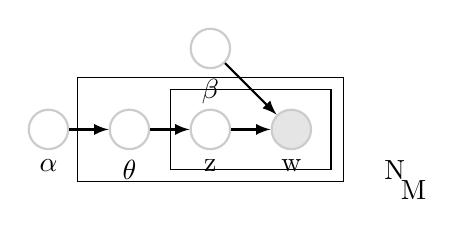
\begin{tikzpicture}
\tikzstyle{main}=[circle, minimum size = 5mm, thick, draw =black!20, node distance = 5mm]
\tikzstyle{connect}=[-latex, thick]
\tikzstyle{box}=[rectangle, draw=black!100]
  \node[main, fill = white!100] (alpha) [label=below:$\alpha$] { };
  \node[main] (theta) [right=of alpha,label=below:$\theta$] { };
  \node[main] (z) [right=of theta,label=below:z] {};
  \node[main] (beta) [above=of z,label=below:$\beta$] { };
  \node[main, fill = black!10] (w) [right=of z,label=below:w] { };
  \path (alpha) edge [connect] (theta)
        (theta) edge [connect] (z)
        (z) edge [connect] (w)
        (beta) edge [connect] (w);
  \node[rectangle, inner sep=0mm, fit= (z) (w),label=below right:N, xshift=13mm] {};
  \node[rectangle, inner sep=2.4mm,draw=black!100, fit= (z) (w)] {};
  \node[rectangle, inner sep=2.6mm, fit= (z) (w),label=below right:M, xshift=12.5mm] {};
  \node[rectangle, inner sep=4mm, draw=black!100, fit = (theta) (z) (w)] {};
\end{tikzpicture}
\vspace{-1em}
\subsubsection{The joint distribution}
$
p(\theta, z, w| \alpha, \beta) = p(\theta | a) \prod_{n=1}^N p(z_n|\theta)p(w_n|z_n,\beta)
$
\subsubsection{The marginal distribution of a document $x$ given the parameters $\alpha$ and $\beta$}
$
p(w|\alpha,\beta) = \int p(\theta|a) \prod_{n=1}^N \sum_{z_n} p(z_n|\theta)p(w_n|z_n,\beta) \mathrm{d}\mathbf{\theta}
$
\subsubsection{The likelihood of the data $D$, $p(D|\alpha,\beta)$}
$
p(D|\alpha,\beta) = \prod_{d=1}^M \int p(\theta_d|\alpha) \prod_{n=1}^{N_d} \sum_{z_{d_n}} p(z_{d_n}|\theta_d)p(w_{d_n}|z_{d_n},\beta) \mathrm{d}\theta_d
$

\subsection{Independent Component Analysis}
We have a set of N observations:\\
$D = \lbrace \mathbf{x}^{(n)} \in \mathbb{R}^J \rbrace ^{N}_{n=1}$\\
, with $I$ independent sources. Thus:\\
$\mathbf{x} = \mathbf{G}\mathbf{s}$, where $G$ is not known. We assume that the latent variables are independently distributed, with marginal distributions $P(s_i|H) = p_i(s_i)$. The probability of the observables and the hidden nodes is:\\
$P(\lbrace x^{(n)},s^{(n)} \rbrace_{n=1}^{N}|G,H) = \prod_{n=1}^N[P(x^{(n)}|s^{(n)},G,H)P(s^{(n)}|H)]$\\
$= \prod_{n=1}^N[(\prod_J \delta(x_j^{(n)} - \sum_i G_{ji}s_i^{(n)}))(\prod_i p_i(s_i^{(n)}))]$.\\ The factor x is generated without noise. For learning the G from the data the likelihood is: $P(D|G,H) = \prod_n P(x^{(n)}|G,H)$\\
, which is a product of factors if we marginalize over the latent variables. We can express each coefficient of $\mathbf{G}$, as a summation over all coefficients multiplied by a delta function such that, $G_{ji}s_i^{(n)} = \sum_i G_{ji}s_i^{(n)}$. ($\mathcal{H}$ denotes the model.)\\
$
p(\mathbf{x^{(n)}} | \mathbf{G}, \mathcal{H}) = \int p(\mathbf{x^{(n)}} | \mathbf{s}^{(n)}, \mathbf{G}, \mathcal{H}) p(\mathbf{s}^{(n)}| \mathcal{H})  \mathrm{d}^I\mathbf{s}^{(n)}\\
= \int \prod_j \delta (x_j^{(n)} - G_{ji}s_i^{(n)}) \prod_i p_i(s_i^{(n)})\mathrm{d}^I\mathbf{s}^{(n)}\\
= \frac{1}{|\det\ \mathbf{G}|} \prod_i p_i(G_{ji}^{-1}x_j) \Rightarrow \\
\ln p(\mathbf{x^{(n)}} | \mathbf{G}, H) = -\ln |\det \mathbf{G}| + \sum_i \ln p_i(G_{ji}^{-1}x_j)
$\\
, which is the log-likelihood of the data D. Now, to find the gradient of the log-likelihood, we are introducing $\mathbf{W} = \mathbf{G}^{-1}$, now the log-likelihood can be written as:\\
$
\ln p(\mathbf{x^{(n)}} | \mathbf{G}, H) = -\ln |\det\mathbf{W}| + \sum_i \ln p_i(W_{ji}x_j)
$\\
The gradient of the log-likelihood equation will be:\\
$
\frac{\partial}{\partial W_{ij}}\ln p(\mathbf{x^{(n)}} | \mathbf{G}, \mathcal{H}) = -\frac{\partial}{\partial W_{ij}}(\ln|\det \mathbf{W}|) + \frac{\partial}{\partial W_{ij}}(\sum_i \ln p_i(W_{ji}x_j))
$

\subsubsection{Factor graph}
Using the computed messages from Bishop book's page $409$, the marginal distribution of variable $x_1$ will be:\\
$ p(x_1) = \mu_{f_a \rightarrow x_1}(x_1)\\
= \sum_{x_2} f_a(x_1,x_2) \mu_{x_2 \rightarrow f_a}(x_2)\\
= \sum_{x_2} f_a(x_1,x_2) \mu_{f_b \rightarrow x_2}(x_2) \mu_{f_c \rightarrow x_2}(x_2)\\
= \sum_{x_2} f_a(x_1,x_2) \sum_{x_3} f_b(x_2,x_3) \sum_{x_4} f_c(x_2,x_4) \\
= \sum_{x_2}\sum_{x_3}\sum_{x_4}  f_a(x_1,x_2) f_b(x_2,x_3) f_c(x_2,x_4)\\
= \sum_{x_2}\sum_{x_3}\sum_{x_4} p(x_1,x_2,x_3,x_4)$
For variable $x_2$ now we have:
$p(x_3) = \mu_{f_b \rightarrow x_3}(x_3)\\
= \sum_{x_2} f_b(x_2,x_3) \mu_{x_2 \rightarrow f_b} (x_2)\\
= \sum_{x_2} f_b(x_2,x_3) \mu_{f_a \rightarrow x_2} (x_2) \mu_{f_c \rightarrow x_2} (x_2)\\
= \sum_{x_2} f_b(x_2,x_3) \sum_{x_1} f_a(x_1,x_2)  \sum_{x_4} f_c(x_2,x_4)\\
= \sum_{x_1} \sum_{x_2} \sum_{x_4}f_b(x_2,x_3)f_a(x_1,x_2) f_c(x_2,x_4)\\
= \sum_{x_1} \sum_{x_2} \sum_{x_4}  p(x_1,x_2,x_3,x_4)
$
Now we are going to show that the sum-product algorithm gives the correct joint distribution for $x_1$ and $x_2$.
$p(x_1, x_2) = f_a(x_1,x_2) \mu_{x_2 \rightarrow f_a}(x_2) \mu_{x_1 \rightarrow f_a(x_1)}\\
= f_a(x_1,x_2) \mu_{x_2 \rightarrow f_a}(x_2),\	\	\	\mu_{x_1 \rightarrow f_a(x_1)} = 1	\\
= f_a(x_1,x_2) \mu_{f_b \rightarrow x_2}(x_2) \mu_{f_c \rightarrow x_2}(x_2)\\
= f_a(x_1,x_2) \sum_{x_3}\sum_{x_4}  f_b(x_2,x_3) f_c(x_2,x_4)\\
= \sum_{x_3}\sum_{x_4}f_a(x_1,x_2) f_b(x_2,x_3) f_c(x_2,x_4)\\
= \sum_{x_3}\sum_{x_4}p(x_1,x_2,x_3,x_4)
$

\subsection{Linear Dynamical Systems}
Transitions: $p(z_n|z_{n-1} = \mathcal{N}(z_n|Az_{n-1}, \Gamma)$ ($\Gamma \rightarrow$ transisition noise)\\
Observations: $p(x_n|z_n) = \mathcal{N}(x_n|Cz_n, \Sigma)$ ($\Sigma \rightarrow$ measurement noise)\\
Initial state: $p(z_1) = \mathcal{N}(z_1|\mu_0, V_0)$. Use EM to learn $A, \Gamma, C, \Sigma, \mu_0, V_0$ \\
$\hat\alpha(z_n) = \mathcal{N}(z_n|\mu_n, V_n)$. \\
$C_n\hat\alpha(z_n) = p(x_n|z_n)\int\hat\alpha(z_{n-1})p(z_n|z_{n-1})dz_{n-1}$. Using 2.115: $c_n = \mathcal{N}(x_n|A\mu_{n-1},\Sigma+CP_{n1}C^T)$. $\mu_n = (P_{n-1}^{-1} + C^T\Sigma^{-1}C)^{-1} (C^T\Sigma^{-1}x_n + P_{n-1}^{-1}A\mu_{n-1})$. $V_n = (P_{n-1}^{-1} + C^T\Sigma^{-1}C)^{-1}$. For stability:\\
$V_n = (I-K_nC)P_{n-1}$; $\mu_n = A\mu_{n-1} + K_n(x_n - CA\mu_{n-1})$ where $x_n-CA\mu_{n-1}$ is the error between observation and expected observation.\\
$c_{n=1}\hat\beta(z_n) = \int \hat\beta(z_{n+1})p(x_{n+1}|z_{n+1}) p(z_{n+1}|z_n) dz_{n+1}$; $\hat\mu_n = \mu_n + J_n(\hat V_{n+1} - P_n)J_n^T$ where $J_n = V_nA^T(P_n)^{-1}$\\
Use $\gamma(z_n) = \hat\alpha(z_n)\hat\beta(z_n) = \mathcal{N}(z_n|\hat\mu_n, \hat V_n)$
Learning: $\text{ln } p(X,Z|\theta) = \text{ln } p(z_1|\mu_0, V_0) + \sum^N_{n=2} \text{ln } p(z_n|z_{n-1}, A, \Gamma) + \sum^N_{n=1} \text{ln } p(x_n|z_n, C, \Sigma)$ \\
$Q(\theta, \theta^{old}) = \mathbb{E}_{z|\theta^{old}}[\text{ln } p(X,Z|\theta)]$.\\
$\mathbb{E}[z_n] = \hat\mu_n$; $\mathbb{E}[z_nz_{n-1}^T] = \hat V_nJ_{n-1}^T+\hat\mu_n\hat\mu_{n-1}^T$; $\mathbb{E}[z_nz_n^T]= \hat V_n + \hat\mu_n\hat\mu_n^T$\\
Kalman gain matrix: $K_n$ as found in $c_n = \mathcal{N}(x_n|\mu_{x_n}, K_n)$

\subsection{Forward-backward for HMM}
$p(x_N|X,z_{N+1}) = p(X_{N+1}, z_{N+1})$\\
$p(z_{N+1}|z_N,X) = p(z_{N+1}, z_N)$ \\
$p(X|z_n) = p(x_1, \ldots, x_n|z_n)p(x_{n+1},\ldots,x_N|z_n)$ \\
$\gamma(z_n) = p(z_n|X) = \frac{p(X|z_n)p(z_n)}{p(X)}$ [$p(X)$ implicitly conditioned on $\theta^{old}$, is likelihood]\\
We can write $\gamma(z_n)=\frac{p(x_1,\ldots,x_n,z_n)p(x_{n+1},\ldots,x_N|z_n)}{p(X)} = \frac{\alpha(z_n)\beta(z_n)}{p(X)}$\\
\textbf{Recursion relations:}\\
$\alpha(z_n) = p(x_n|z_n)\sum_{z_{n-1}} \alpha(z_{n-1})p(z_n|z_{n-1})$\\
$\alpha(z_1) = p(x_1,z_1) = p(z_1)p(x_1|z_1) = \prod^K_{k=1} \{\pi_kp(x_1|\phi_k)\}^{z_{1k}}$\\
$\beta(z_n) = \sum_{z_{n+1}} \beta(z_{n+1})p(x_{n+1}|z_{n+1})p(z_{n+1}|z_n)$\\
$\beta(z_N) = 1 $\\
$\xi(z_{n-1},z_n) = p(z_{n-1},z_n|X) = \frac{\alpha(z_{n-1})p(x_n|z_n)p(z_n|z_{n-1})\beta(z_n)}{p(X)}$
\textbf{Joint}\\
$p(X) = \sum_{z_n}\alpha(z_n)\beta(z_n)$\\
\textbf{EM}:\\
E-step: Evaluate $\gamma(z_n)$ and $\xi(z_{n-1},z_n)$. M-step: maximize $Q(\theta,\theta^{old}) = \sum_Z p(Z|X,\theta^{old}) \text{ln } p(X,Z|\theta)$
$= \sum^K_{k=1} \gamma(z_{1k}) \text{ln }\pi_k + \sum^N_{n=2}\sum^K_{j=1}\sum^K_{k=1} \xi(z_{n-1,j}z_{nk})\text{ln }A_{jk} + \sum^N_{n=1}\sum^K_{k=1}\gamma(z_{nk})\text{ln } p(x_n|\phi_k)$
\subsection{Sum-product for HMM}
We define:\\
$h(z_1) = p(z_1)p(x_1|z_1)$\\
$f_n(z_{n-1},z_n) = p(z_n|z_{n-1})p(x_n|z_n)$\\
Define final hidden variable $z_n$ as root, and first pass from h to root:\\
$\mu_{z_{n-1}\rightarrow f_n}(z_{n-1}) = \mu_{f_{n-1}\rightarrow z_{n-1}}(z_{n-1})$\\
$\mu_{f_n\rightarrow z_n}(z_n) = \sum_{z_{n-1}}f_n(z_{n-1},z_n) \mu_{z_{n-1} \rightarrow f_n}(z_{n-1})$\\
We can set:\\
$\alpha(z_n) = \mu_{f_n\rightarrow z_n}(z_n)$\\
Next, we propagate from the root back to the leaf:\\
$\mu_{f_{n+1}\rightarrow f_n}(z_n) = \sum_{z_{n+1}} f_{n+1}(z_n,z_{n+1}) \mu_{f_{n+1}\rightarrow f_{n+1}}(z_{n+1})$\\
And we can set:\\
$\beta(z_n) = \mu_{f_{n+1}\rightarrow z_n}(z_n)$

\subsection{Factorized distributions in approx inf}
$\mathcal{L}(q) = \int \prod_i q_i \big\{ \text{ln } p(X,Z) - \sum_i \text{ln } q_i \}dZ$\\
$= \int q_j \mathbb{E}_{i\not=j}[\text{ln } p(X,Z)] + \text{const}$\\
$\mathbb{E}_{i\not=j}[\text{ln }p(X,Z)] = \int \text{ln }p(X,Z) \prod_{i\not=j}q_idZ_i$\\
$q_j^* = \frac{\text{exp} (\mathbb{E}_{i\not=j} [\text{ln }p(X,Z)] ) }{\int \text{exp} (\mathbb{E}_{i\not=j} [\text{ln }p(X,Z)] ) dZ_j}$

\subsection{Joint Prob. in BN}
The joint probability over all the nodes in a BN is:
$
p(x_1,x_2,\ldots,x_k) = p(x_k|\mathrm{pa}_k) \times p(x_{k-1}|\mathrm{pa}_{k-1})\times \ldots p(x_1|\emptyset)
$
, where $\mathrm{pa}_i$ parents of node $i$, and node $1$ the root node. Assuming that the level of each node is proportional to each subscript, we can marginalize over the nodes of the deepest levels.
$
\sum_{x_1}p(x_1,x_2,\ldots,x_k) \ldots \sum_{x_K}p(x_1,x_2,\ldots,x_k) =\\
\sum_{x_1}p(x_1| \emptyset ) \ldots \sum_{x_K}p(x_K|\mathrm{pa}_K) \prod_{j=1}^{K-1}p(x_j|\mathrm{pa}_j) =\\
$
Provided that the individual conditional distributions are normalized and the term $x_K$ is not affecting the other terms in the above equation, Recursively we eliminate all variable, ending up in: $\sum_x\prod_{k=1}^kp(x_k|\mathrm{pa}_k) =1$
\vspace{.5em}
\section{Mathematical Tricks}
\vspace{-.5em}
$-\frac{1}{2}(x-\mu)^\top\Sigma^{-1}(x-\mu) = -\frac{1}{2}x^\top \Sigma^{-1}x + x^\top \Sigma^{-1} \mu + c$\\
$\frac{\partial a^\top X b}{\partial X} = ab^\top$,
$\frac{\partial a^\top X^\top b}{\partial X} = ba^\top$\\
$\frac{\partial \det X}{\partial X} = \det (X) (X^{-1})^\top$ \\
$M = M^\top \iff u^\top M v = v^\top M u$\\
$\mathbb{E}[(x-\mu)^\top \Sigma^{-1} (x-\mu)\mathcal{N}(x|\mu, \Sigma)] = \mathrm{Tr}(\Sigma^{-1}\Sigma) = D$\\
$\mathbb{E} [x] = \int^\infty_{-\infty}x f(x)\mathrm{d}x$\\
Product of Gaussians: $\Sigma = (\Sigma_1^{-1} + \Sigma_2^{-1})^{-1}$, $\mu = \Sigma \Sigma_1^{-1} \mu_1 + \Sigma \Sigma_2^{-1} \mu_2$\\
Other: $(P^{-1}+B^\top R^{-1}B)^{-1}B^\top R^{-1} = PB^\top (BPB^\top + R)^{-1}$\\
Woodbury: $(A+BD^{-1}C)^{-1} = A^{-1} - A^{-1}B(D+CA^{-1}B)^{-1}CA^{-1}$\\
Gradient in exp family wrt for $\eta$, for $p(x|\eta) = h(x)g(\eta)\text{exp}\{\eta^Tu(x)\}$, where $g(\eta)\int h(x) \text{exp}\{\eta^Tu(x)\} dx = 1$, we have the result:$- \nabla \text{ln } g(\eta) = \mathbb{E}[u(x)]$
\end{multicols}
\end{document}
